\Chapter{Benutzerschnittstelle}

Im Folgenden wird die Benutzung des auf dem FPGA realisierten RISC-V Prozessors geschildert, wobei im Besonderen auf die Nutzerschnittstelle eingegangen wird. Um das FPGA in Betrieb zu nehmen, muss dieses logischerweise an eine entsprechende Stromquelle angeschlossen sein.

\Section{Initialisierung}

Im Allgemeinen kann ein Assemblerprogramm, das aus den implementierten Instruktionen zusammengesetzt ist, auf zwei Weisen in den Programmspeicher geladen und dann auf dem Prozessor ausgef\"uhrt werden.

\Subsection{Initialisierung durch BIOS und serielle Schnitstelle}

Die Programm-Einsprungsadresse, bei welcher die CPU die Ausf\"uhrung nach Beendigung eines Resets beginnt, Befehle abzuarbeiten, ist die erste Adresse des BIOS-RAM-Blocks \textit{0x00000000}. Dieser RAM-Block wird provisorisch mit einem einfachen BIOS-Programmcode initialisiert:


\begin{lstlisting}
	lui x1, 0x40000
	jalr x0, x1, 0
\end{lstlisting}

Dieser Programmcode f\"uhrt  die Ausf\"uhrung in einem anderen RAM-Block fort, dem SERIALRAM, welcher durch das Pr\"afix 0x4 auf die Speicheradresse \textit{0x40000000} gemappt ist. Der Programmierer muss zuvor also gew\"ahrleisten, dass dieser Speicherbereich, welcher durch die serielle Schnittstelle UART gef\"ullt wird, mit ausf\"uhrbarem Programmcode initialisiert wurde.

Indem der Programmierer nach einem Reset den Programmstart bei oben erw\"ahnter Einsprungsadresse durch das Halten des entsprechenden Blockadesignals auf Switch 4 (siehe Abbildung \ref{fig:pinning}) verz\"ogert, bleibt Zeit w\"ahrenddessen \"uber die UART Schnittstelle den SERIALRAM-Speicherblock zu initialisieren. Indem das Signal auf Switch 4 wieder entfernt wird, beginnt der Programmablauf wie eingangs erw\"ahnt im BIOS-RAM.
Da die serielle Schnittstelle nur f\"ur begrenzte Datenmengen verl\"asslich und fehlerfrei funktioniert, k\"onnen keine gr\"o\ss{}eren Programme auf diese Weise ausgef\"uhrt werden.

\Subsection{Initialisierung durch initiales Beschreiben des BIOS-RAM Blocks}

Alternativ besteht auch die M\"oglichkeit, den BIOS-RAM Block direkt beim Beschreiben des FPGAs mit dem auszuf\"uhrenden Programmcode zu initialisieren. Da der BIOS-RAM-Block als Dual-Port-Blockram realisiert wurde, kann dies ohne zeitlichen Aufwand bei einem Reset erfolgen.

Das BIOS wird auf diese Weise zweckentfremdet und der SERIALRAM Block bleibt ungenutzt. Auch muss das FPGA zur Ausf\"uhrung eines anderen Programms jedes Mal neu beschrieben werden. Trotz der genannten Nachteile aber bleibt diese Methode vorerst die einzig verl\"assliche Vorgehensweise, auch gr\"o\ss{}ere Datenmengen auf das Board zu \"ubertragen. Sie findet beispielsweise im Fall des sp\"ater beschriebenen Demoprogramms Anwendung.

\Section{Der Reset}

Nachdem das FPGA mit entsprechender Methodik initialisiert wurde oder aber nachdem eine Programmausf\"uhrung terminiert hat, muss der Prozessor zur\"uckgesetzt werden. Dies geschieht durch das kurzzeitige Halten des Reset-Signals, welches auf den Hardware-Switch \textit{SW 0} (siehe Abbildung \ref{fig:pinning}) gemappt ist.

Zu beachten ist, dass der Reset nur im verlangsamten Ausf\"uhrungsmodus (5 Hz) verl\"asslich funktioniert. Ob ein Reset im schnellen Ausf\"uhrungsmodus (50 MHz) erfolgreich verl\"auft, ist nichtdeterministisch und daher auch nicht zu empfehlen.

\Section{Graphische Oberfl\"achen}

Im Allgemeinen existieren zwei Methoden die Programmausf\"uhrung graphisch darzustellen: Einerseits existiert der Debugging-Modus, in welchem die Werte aller verf\"ugbaren Register sowie des Programmz\"ahlers und des Instruktionsregisters ausgegeben werden. Andererseits wird gleichzeitig der Speicherbereich des CHARRAM-Blocks auf eine ASCII-Darstellung gemappt. Mittels des Hardware-Switches \textit{SW 2} (siehe Abbildung \ref{fig:pinning}) wird bestimmt, welcher der beiden Modi auf dem VGA-Ausgang ausgegeben wird. Dabei bedeutet ein Halten des Switches die Darstellung \"uber ASCII und ein Loslassen die direkte Ausgabe der Register innerhalb der CPU.

\Subsection{Debugging-Modus}

Der Debugging-Modus zeichnet die verf\"ugbaren 32 Register x0-x31 bitweise auf das VGA-Ausgabeger\"at. Dabei werden die Register farblich voneinander getrennt und zeilenweise fortlaufend durchnummeriert (pro Zeile vier Register). Gesetzte Balken entsprechen einem gesetzten Bit innerhalb des Registerwerts, wobei das \textit{least significant Bit} links, und das \textit{most significant Bit} rechts dargestellt wird.
Die beiden separat dargestellten Register sind der Programmz\"ahler (links) sowie das Instruktionsregister (rechts), ebenfalls bitweise abgebildet.

\begin{figure}[H]
	\centering
	\label{fig:debuggingui}
		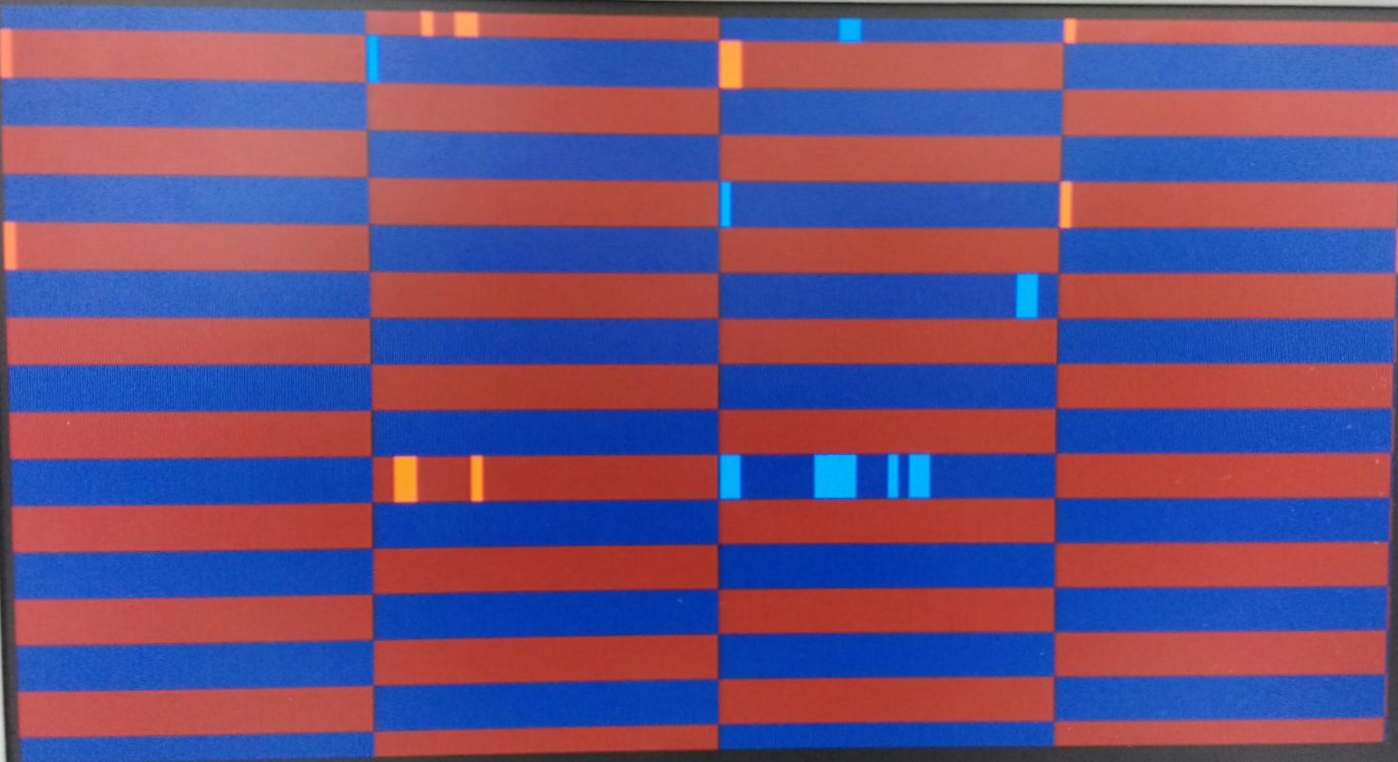
\includegraphics[width=0.4\textwidth]{debugui.png}
	\caption[VGA-Ausgabe im Debugging-Modus]{VGA-Ausgabe im Debugging-Modus: PC und IR liegen zentral}
\end{figure}

Da die VGA-Ausgabe mit 25 MHz getaktet wird, der Prozessor im schnellen Ausf\"uhrungsmodus dagegen den vielfachen Takt erh\"alt, wechseln die Registerwerte unter Umst\"anden schneller, als sie dargestellt werden k\"onnen, wodurch es zu signifikanten Darstellungsfehlern kommen kann. Der Debugging-Modus ist dementsprechend, wie der Name bereits suggeriert lediglich f\"ur Debugging-Zwecke im langsamen Ausf\"uhrungsmodus sinnvoll nutzbar.

\Subsection{ASCII-Modus}
Der ASCII-Modus stellt zeilenweise fortlaufend durchnummeriert die Werte der Speicherzellen innerhalb des CHAR\-RAM-Blocks als ASCII-Zeichen dar. Die genaue Abbildungsmethodik wird in Kapitel \ref{ch:asciiunit} n\"aher erl\"autert.

Um das Demo-Programm sinnvoll zu benutzten, wird dieser Ausf\"uhrungsmodus empfohlen, da er einerseits auch im schnellen Ausf\"uhrungsmodus aufgrund der Seltenheit von schreibenden Speicherzugriffen im entsprechenden CHAR\-RAM-Block konsistenter Daten anzeigt, und andererseits das Programm so konzipiert ist, dass das Tic-Tac-Toe Spiel die ASCII-Schnittstelle zur Benutzerinteraktion vorsieht.

\Section{Benutzereingabe}

Analog zur Ausgabe von Daten bietet der Prozessor auch eine M\"oglichkeit zur Dateneingabe durch den Benutzer. Wie in Kapitel \ref{sec:mmuio} genauer erl\"autert wird, sind alle Buttons, Switches und LEDs auf Speicherzellen gemappt. Ein Halten oder Loslassen der entsprechenden Komponente f\"uhrt zu einem Wechsel des Bits an entsprechender Speicheradresse.

Programmierer haben so die M\"oglichkeit Benutzereingaben abzufragen oder auf diese zu reagieren, m\"ussen das aber innerhalb ihrer Implementierung selbst tun, da keinerlei Interrupts oder dergleichen bereitgestellt werden.

\newpage

